
\section{数组回顾}

\begin{frame}[fragile]\ft{数组}
数组由一系列类型相同的元素组成,数组声明必须包括元素的个数(即数组长度)与类型。如

\begin{lstlisting}
float farray[20];
char carray[12];
int iarray[50];
\end{lstlisting}
\end{frame}

\begin{frame}[fragile]\ft{数组初始化}
\begin{figure}
\centering
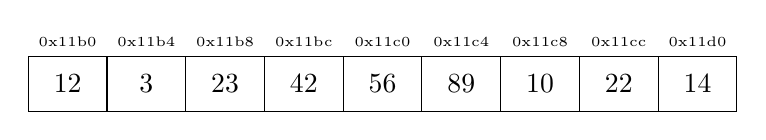
\begin{tikzpicture}
\draw (0,0) rectangle node[] {12} (1,0.7); \node at (0.5,0.7) [above] {\tf \tiny 0x11b0};
\draw (1,0) rectangle node[] {3} (2,0.7);  \node at (1.5,0.7) [above] {\tf \tiny 0x11b4};
\draw (2,0) rectangle node[] {23} (3,0.7); \node at (2.5,0.7) [above] {\tf \tiny 0x11b8};
\draw (3,0) rectangle node[] {42} (4,0.7); \node at (3.5,0.7) [above] {\tf \tiny 0x11bc};
\draw (4,0) rectangle node[] {56} (5,0.7); \node at (4.5,0.7) [above] {\tf \tiny 0x11c0};
\draw (5,0) rectangle node[] {89} (6,0.7); \node at (5.5,0.7) [above] {\tf \tiny 0x11c4};
\draw (6,0) rectangle node[] {10} (7,0.7); \node at (6.5,0.7) [above] {\tf \tiny 0x11c8};
\draw (7,0) rectangle node[] {22} (8,0.7); \node at (7.5,0.7) [above] {\tf \tiny 0x11cc};
\draw (8,0) rectangle node[] {14} (9,0.7); \node at (8.5,0.7) [above] {\tf \tiny 0x11d0};
\end{tikzpicture}
\end{figure}

$$
\Big\downarrow  \mbox{\lstinline|int array[5];|}
$$


\begin{figure}
\centering
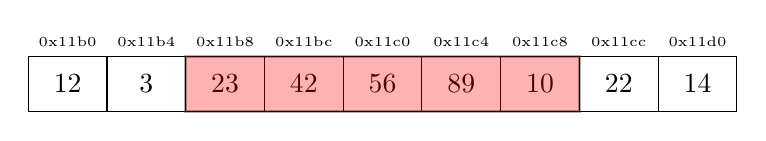
\begin{tikzpicture}
\draw (0,0) rectangle node[] {12} (1,0.7); \node at (0.5,0.7) [above] {\tf \tiny 0x11b0};
\draw (1,0) rectangle node[] {3} (2,0.7);  \node at (1.5,0.7) [above] {\tf \tiny 0x11b4};
\draw (2,0) rectangle node[] {23} (3,0.7); \node at (2.5,0.7) [above] {\tf \tiny 0x11b8};
\draw (3,0) rectangle node[] {42} (4,0.7); \node at (3.5,0.7) [above] {\tf \tiny 0x11bc};
\draw (4,0) rectangle node[] {56} (5,0.7); \node at (4.5,0.7) [above] {\tf \tiny 0x11c0};
\draw (5,0) rectangle node[] {89} (6,0.7); \node at (5.5,0.7) [above] {\tf \tiny 0x11c4};
\draw (6,0) rectangle node[] {10} (7,0.7); \node at (6.5,0.7) [above] {\tf \tiny 0x11c8};
\draw (7,0) rectangle node[] {22} (8,0.7); \node at (7.5,0.7) [above] {\tf \tiny 0x11cc};
\draw (8,0) rectangle node[] {14} (9,0.7); \node at (8.5,0.7) [above] {\tf \tiny 0x11d0};

\draw[opacity=0.3, fill=red, very thick] (2,0) rectangle (7,0.7);
\end{tikzpicture}
\end{figure}


\pause 

{\bf 数组名表示的是数组首元素的地址。故\lstinline| array |的值为\lstinline| 0x11b8 |。}

\end{frame}


\begin{frame}[fragile]\ft{数组初始化}
\begin{figure}
\centering
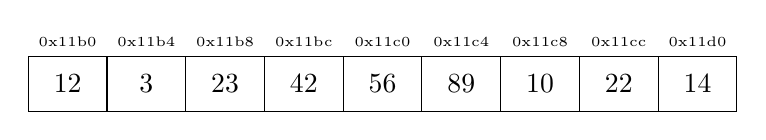
\begin{tikzpicture}
\draw (0,0) rectangle node[] {12} (1,0.7); \node at (0.5,0.7) [above] {\tf \tiny 0x11b0};
\draw (1,0) rectangle node[] {3} (2,0.7);  \node at (1.5,0.7) [above] {\tf \tiny 0x11b4};
\draw (2,0) rectangle node[] {23} (3,0.7); \node at (2.5,0.7) [above] {\tf \tiny 0x11b8};
\draw (3,0) rectangle node[] {42} (4,0.7); \node at (3.5,0.7) [above] {\tf \tiny 0x11bc};
\draw (4,0) rectangle node[] {56} (5,0.7); \node at (4.5,0.7) [above] {\tf \tiny 0x11c0};
\draw (5,0) rectangle node[] {89} (6,0.7); \node at (5.5,0.7) [above] {\tf \tiny 0x11c4};
\draw (6,0) rectangle node[] {10} (7,0.7); \node at (6.5,0.7) [above] {\tf \tiny 0x11c8};
\draw (7,0) rectangle node[] {22} (8,0.7); \node at (7.5,0.7) [above] {\tf \tiny 0x11cc};
\draw (8,0) rectangle node[] {14} (9,0.7); \node at (8.5,0.7) [above] {\tf \tiny 0x11d0};
\end{tikzpicture}
\end{figure}

$$
\Big\downarrow  \mbox{\lstinline|int array[5] = {1,2,3};|}
$$


\begin{figure}
\centering
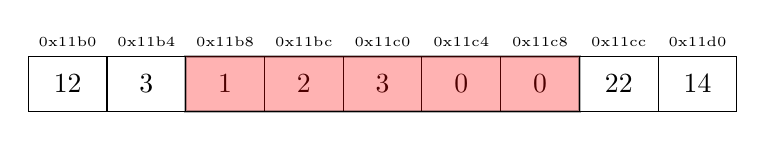
\begin{tikzpicture}
\draw (0,0) rectangle node[] {12} (1,0.7); \node at (0.5,0.7) [above] {\tf \tiny 0x11b0};
\draw (1,0) rectangle node[] {3} (2,0.7);  \node at (1.5,0.7) [above] {\tf \tiny 0x11b4};
\draw (2,0) rectangle node[] {1} (3,0.7); \node at (2.5,0.7) [above] {\tf \tiny 0x11b8};
\draw (3,0) rectangle node[] {2} (4,0.7); \node at (3.5,0.7) [above] {\tf \tiny 0x11bc};
\draw (4,0) rectangle node[] {3} (5,0.7); \node at (4.5,0.7) [above] {\tf \tiny 0x11c0};
\draw (5,0) rectangle node[] {0} (6,0.7); \node at (5.5,0.7) [above] {\tf \tiny 0x11c4};
\draw (6,0) rectangle node[] {0} (7,0.7); \node at (6.5,0.7) [above] {\tf \tiny 0x11c8};
\draw (7,0) rectangle node[] {22} (8,0.7); \node at (7.5,0.7) [above] {\tf \tiny 0x11cc};
\draw (8,0) rectangle node[] {14} (9,0.7); \node at (8.5,0.7) [above] {\tf \tiny 0x11d0};
\draw[opacity=0.3, fill=red, very thick] (2,0) rectangle (7,0.7);
\end{tikzpicture}
\end{figure}

\end{frame}


\begin{frame}[fragile]\ft{数组初始化}
\begin{figure}
\centering
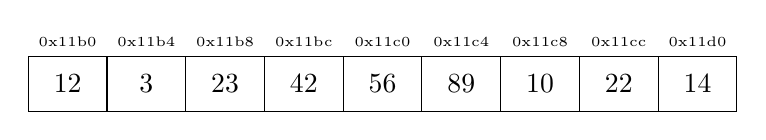
\begin{tikzpicture}
\draw (0,0) rectangle node[] {12} (1,0.7); \node at (0.5,0.7) [above] {\tf \tiny 0x11b0};
\draw (1,0) rectangle node[] {3} (2,0.7);  \node at (1.5,0.7) [above] {\tf \tiny 0x11b4};
\draw (2,0) rectangle node[] {23} (3,0.7); \node at (2.5,0.7) [above] {\tf \tiny 0x11b8};
\draw (3,0) rectangle node[] {42} (4,0.7); \node at (3.5,0.7) [above] {\tf \tiny 0x11bc};
\draw (4,0) rectangle node[] {56} (5,0.7); \node at (4.5,0.7) [above] {\tf \tiny 0x11c0};
\draw (5,0) rectangle node[] {89} (6,0.7); \node at (5.5,0.7) [above] {\tf \tiny 0x11c4};
\draw (6,0) rectangle node[] {10} (7,0.7); \node at (6.5,0.7) [above] {\tf \tiny 0x11c8};
\draw (7,0) rectangle node[] {22} (8,0.7); \node at (7.5,0.7) [above] {\tf \tiny 0x11cc};
\draw (8,0) rectangle node[] {14} (9,0.7); \node at (8.5,0.7) [above] {\tf \tiny 0x11d0};
\end{tikzpicture}
\end{figure}

$$
\Big\downarrow  \mbox{\lstinline|int array[5] = {2, [2]=5, 6, [0]=8};|}
$$


\begin{figure}
\centering
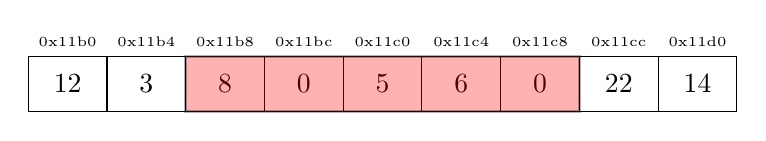
\begin{tikzpicture}
\draw (0,0) rectangle node[] {12} (1,0.7); \node at (0.5,0.7) [above] {\tf \tiny 0x11b0};
\draw (1,0) rectangle node[] {3} (2,0.7);  \node at (1.5,0.7) [above] {\tf \tiny 0x11b4};
\draw (2,0) rectangle node[] {8} (3,0.7); \node at (2.5,0.7) [above] {\tf \tiny 0x11b8};
\draw (3,0) rectangle node[] {0} (4,0.7); \node at (3.5,0.7) [above] {\tf \tiny 0x11bc};
\draw (4,0) rectangle node[] {5} (5,0.7); \node at (4.5,0.7) [above] {\tf \tiny 0x11c0};
\draw (5,0) rectangle node[] {6} (6,0.7); \node at (5.5,0.7) [above] {\tf \tiny 0x11c4};
\draw (6,0) rectangle node[] {0} (7,0.7); \node at (6.5,0.7) [above] {\tf \tiny 0x11c8};
\draw (7,0) rectangle node[] {22} (8,0.7); \node at (7.5,0.7) [above] {\tf \tiny 0x11cc};
\draw (8,0) rectangle node[] {14} (9,0.7); \node at (8.5,0.7) [above] {\tf \tiny 0x11d0};

\draw[opacity=0.3, fill=red, very thick] (2,0) rectangle (7,0.7);
\end{tikzpicture}
\end{figure}

\end{frame}


\section{指针}
\begin{frame}[fragile]\ft{\secname}
\begin{itemize}
\item
计算机的硬件指令很大程度上依赖于地址,而指针为我们使用地址提供了一种方法。\\[0.1in]
\item
使用指针能让我们以类似于计算机底层的方式来表达意愿,从而让程序能更高效地工作。\\[0.1in]
\item 
需要强调的是,指针能非常有效地处理数组。事实上,\red{数组是一种变相使用指针的形式。}
\end{itemize}
\end{frame}


\begin{frame}[fragile]\ft{\secname}
再一次强调:\red{数组名是数组首元素的地址。}
\pause \vspace{0.2in}

若\lstinline| array |为一个数组,则以下关系式为真:
\begin{lstlisting}[language=c,backgroundcolor=\color{red!20}]
array == &array[0];
\end{lstlisting}
\end{frame}


\begin{frame}[fragile,allowframebreaks]\ft{\secname}
  \lstinputlisting
  [language=c,numbers=left,frame=single]
  {ch10/code/pnt_add.c}
\end{frame}


\begin{frame}[fragile]\ft{\secname}

\begin{lstlisting}[backgroundcolor=\color{red!20}]
               short double
pointers + 0: 0xf7d0 0xf7b0
pointers + 1: 0xf7d2 0xf7b8
pointers + 2: 0xf7d4 0xf7c0
pointers + 3: 0xf7d6 0xf7c8
\end{lstlisting}
\end{frame}


\begin{frame}[fragile]\ft{\secname}
在C中,对指针加1的结果是对该指针增加一个存储单元。对数组而言,地址会增加到下一个元素的地址,而不是下一个字节。
\end{frame}


\begin{frame}[fragile]\ft{\secname}
\begin{center}
\red{\Large 指针定义小结}
\end{center}
\begin{itemize}
\item 
指针的数值就是它所指向的对象的地址。地址的内部表达方式由硬件决定,很多计算机都是以字节编址的。 \\[0.1in]
\item
在指针前用运算符\lstinline| * |就可以得到该指针所指向的对象的值。\\[0.1in]
\item
对指针加1,等价于对指针的值加上它所指向的对象的字节大小。
\end{itemize}
\end{frame}


\begin{frame}[fragile]\ft{\secname}
\begin{lstlisting}[language=c,backgroundcolor=\color{red!20}]
dates + 2 == &dates[2];    // same address
*(dates + 2) == dates[2];  // same value
\end{lstlisting}

可以用指针标识数组的每个元素,并得到每个元素的值。从本质上讲,这是对同一对象采用了两种不同的符号表示方法。

\end{frame}


\begin{frame}[fragile]\ft{\secname}
在描述数组时,C确实借助了指针的概念。例如,定义\lstinline| array[n] |时,\vspace{0.1in}

\begin{itemize}
\item
即:\lstinline| *(array + n) |, \\[0.1in]
\item
含义:“寻址到内存中的\lstinline| array |,然后移动\lstinline| n |个单元,再取出数值”。
\end{itemize}
\end{frame}


\begin{frame}[fragile]\ft{\secname}
请注意\lstinline| *(dates+2) |和\lstinline| *dates+2 |的区别。\red{取值运算符\lstinline| * |的优先级高于\lstinline| + |},故后者等价于\lstinline| (*dates)+2 |。\vspace{0.1in}

\begin{lstlisting}[language=c,backgroundcolor=\color{red!20}]
*(dates + 2)  //  same as dates[2]
*dates + 2    //  same as dates[0] + 2
\end{lstlisting}
\end{frame}
 

\section{数组、指针与函数}

\begin{frame}[fragile]\ft{\secname}
编写函数,求一个数组的各元素之和。
\end{frame}

\begin{frame}[fragile]\ft{\secname}
方式一:在函数中给定固定的数组大小。
\begin{lstlisting}[language=c,backgroundcolor=\color{red!20}]
int sum(int * ar)
{
  int i, total = 0;
  
  for (i = 0; i < 10; i++)
    total += ar[i];  
  return total;  
}
\end{lstlisting} \pause 
但该函数仅在数组长度为10时可工作。
\end{frame}

\begin{frame}[fragile]\ft{\secname}
方式二:将数组大小作为参数传递给函数。
\begin{lstlisting}[language=c,backgroundcolor=\color{red!20}]
int sum(int * ar, int n)
{
  int i, total = 0;
  
  for (i = 0; i < n; i++)
    total += ar[i];  
  return total;  
}
\end{lstlisting} \pause 
该方式更为灵活,第一个参数把数组地址和数组类型的信息传递给函数,第二个参数把数组的元素个数传递给函数。
\end{frame}

\begin{frame}[fragile]\ft{\secname}
给定数组
\begin{lstlisting}[language=c,backgroundcolor=\color{red!20},frame=no]
int ar[5] = {1, 2, 3, 4, 5};
\end{lstlisting}
\begin{itemize}
\item 可以求数组的整体和,如
\begin{lstlisting}[language=c,backgroundcolor=\color{red!20},frame=no]
int result = sum(ar, 5);
\end{lstlisting}
\item 也可以求数组的部分和,如
\begin{lstlisting}[language=c,backgroundcolor=\color{red!20},frame=no]
int result = sum(ar+1, 3);
\end{lstlisting}
计算的是\lstinline|ar|的第2个至第4个元素之和。
\end{itemize}

\end{frame}




\begin{frame}[fragile]\ft{\secname}
在做函数声明时,以下四种函数原型是等价的:
\begin{lstlisting}[language=c,backgroundcolor=\color{red!20}]
int sum(int * ar, int n);
int sum(int *, int);

int sum(int ar[], int n);
int sum(int [], int);
\end{lstlisting}
\end{frame}

\begin{frame}[fragile]\ft{\secname}
在定义函数时,名称不可以省略。故在定义时以下两种形式是等价的:
\begin{lstlisting}[language=c,backgroundcolor=\color{red!20}]
int sum(int * ar, int n)
{
  ...
}

int sum(int ar[], int n)
{
  ...
}
\end{lstlisting}
\end{frame}

